% ============================================================
% CHAPTER 2: LITERATURE REVIEW
% ============================================================
\chapter{Literature Review}
\label{ch:literature}

This chapter reviews the literature underpinning a standards-based, network-level cycling assessment. Section~\ref{sec:lit-background} establishes why infrastructure provision shapes participation, locating the mechanism in perceived safety and uneven stress tolerance. Section~\ref{sec:lit-ltn} examines LTN 1/20 and the limits of its scheme-level instruments. Section~\ref{sec:lit-lts} introduces the Level of Traffic Stress framework and its applications. Section~\ref{sec:lit-networkgrowth} reviews network growth simulation. Section~\ref{sec:lit-gaprq} identifies the resulting gaps and states the research questions.

\section{Infrastructure Quality, Perceived Safety, and Cycling Participation}
\label{sec:lit-background}

The widely reported positive association between infrastructure provision and cycling participation raises a prior question of why provision should exert this influence \parencite{hull2014,pistoll2014,buehler2016,molenberg2019}. A substantial body of work answers this by locating the mechanism in safety, and more precisely in its subjective dimension: whereas objective safety concerns the recorded incidence of crashes and injuries, it is the perceived safety, or how safe cycling is felt to be, that most directly shapes the decision to cycle, particularly for prospective and occasional riders \parencite{chaurand2013,sanders2015,manton2016}. This distinction between objective and subjective safety is what the language of traffic stress was introduced to capture. Early work characterised the discomfort imposed on a cyclist by the speed, volume, and proximity of adjacent motor traffic as a graded property of the road environment rather than a binary of safe and unsafe \parencite{sorton1994,landis1997,harkey1998}. Framed this way, the stress a cyclist experiences is understood as a systematic response to the traffic conditions a facility exposes them to, so that it can be inferred from the road's physical and operational characteristics rather than measured directly. The value of the concept is that it makes the deterrent effect of traffic legible in terms of design variables that infrastructure can be built to modify.

Critically, tolerance of this stress is not uniform across the population. Stated-preference studies consistently find that groups currently under-represented among cyclists, women in particular, express stronger preferences for separation from motor traffic than men, with weaker but converging evidence for older adults and for those cycling with children \parencite{aldred2017}. The latent demand that infrastructure investment seeks to convert is therefore concentrated precisely among those least willing to tolerate high-stress conditions. This population corresponds to the widely reported “interested but concerned” segment, individuals who would consider cycling if protected from stressful traffic environments and who represent the largest and most winnable constituency for mode shift \parencite{geller2009,mekuria2012a,dill2013}. Consequently, the relevant question is not only whether provision works for those already riding in traffic, but whether it also extends to the stress-averse users at the other end of the spectrum, on whom further uptake depends.

The relationship between perceived safety and cycling participation cannot be understood solely from the characteristics of individual links. Route choice evidence consistently shows that cyclists are willing to accept substantial detours to avoid stressful links and crossings \parencite{broach2012,park2019,berghoefer2023}, indicating that routes are evaluated as integrated wholes rather than as collections of independent facilities. Where no acceptable alternative exists, a single hostile link or crossing becomes a bottleneck that can render an otherwise suitable route unacceptable \parencite{mekuria2012a,furth2016,furth2018}. It follows that the infrastructure quality relevant to the stress-averse majority is a property of connected networks rather than of individual facilities, and that its assessment requires criteria referenced to the populations expected to use them, applied to whole journeys rather than isolated schemes.



\section{LTN 1/20: Design Standards for Cycling Infrastructure in England}
\label{sec:lit-ltn}

\textit{``A travel revolution in our streets, towns and communities will have made cycling a mass form of transit. Cycling and walking will be the natural first choice for many journeys with half of all journeys in towns and cities being cycled or walked by 2030''}
\parencite{departmentfortransport2020}.

This ambitious goal, set out in the Gear Change white paper, marked an unprecedented elevation in UK active travel policy. To translate this political commitment into consistent design practice, the Department for Transport simultaneously published Local Transport Note 1/20 (LTN 1/20), the most comprehensive national guidance for cycling infrastructure design and assessment to date \parencite{departmentfortransport2020a}. To cater for the broadest range of cyclists and deliver on Gear Change's ambition of mass cycling uptake, LTN 1/20 establishes as first principle that cycle infrastructure should be accessible to everyone “from 8 to 80 and beyond”, with inclusive design running through all aspects of implementation \parencite{departmentfortransport2020a}. 

To assess whether infrastructure meets this standard, LTN 1/20 organises its evaluation framework around five core design principles derived from Dutch practice \parencite{crow2016} — Coherence, Directness, Safety, Comfort, and Attractiveness — and introduced two complementary assessment instruments. The Cycling Level of Service (CLoS) tool appraises link-level attributes across 25 subcriteria under these five principles, each scored 0-2 with designated critical failures that override the overall assessment; the Junction Assessment Tool (JAT) complements CLoS at junctions, with its three scoring tiers explicitly anchored to distinct user populations (Figure~\ref{fig:ltn}). With the establishment of Active Travel England (ATE) as the national inspectorate in 2022, these instruments became central to a formal compliance process: only schemes achieving a minimum CLoS score of 70\%, with no critical failures and no red-scored turning movements under the JAT, are generally considered eligible for Active Travel Fund allocations \parencite{departmentfortransport2020a}. This mechanism has effectively transformed LTN 1/20 from advisory guidance into a binding quality threshold for publicly funded cycling infrastructure.

\begin{figure}[htbp]
    \centering
    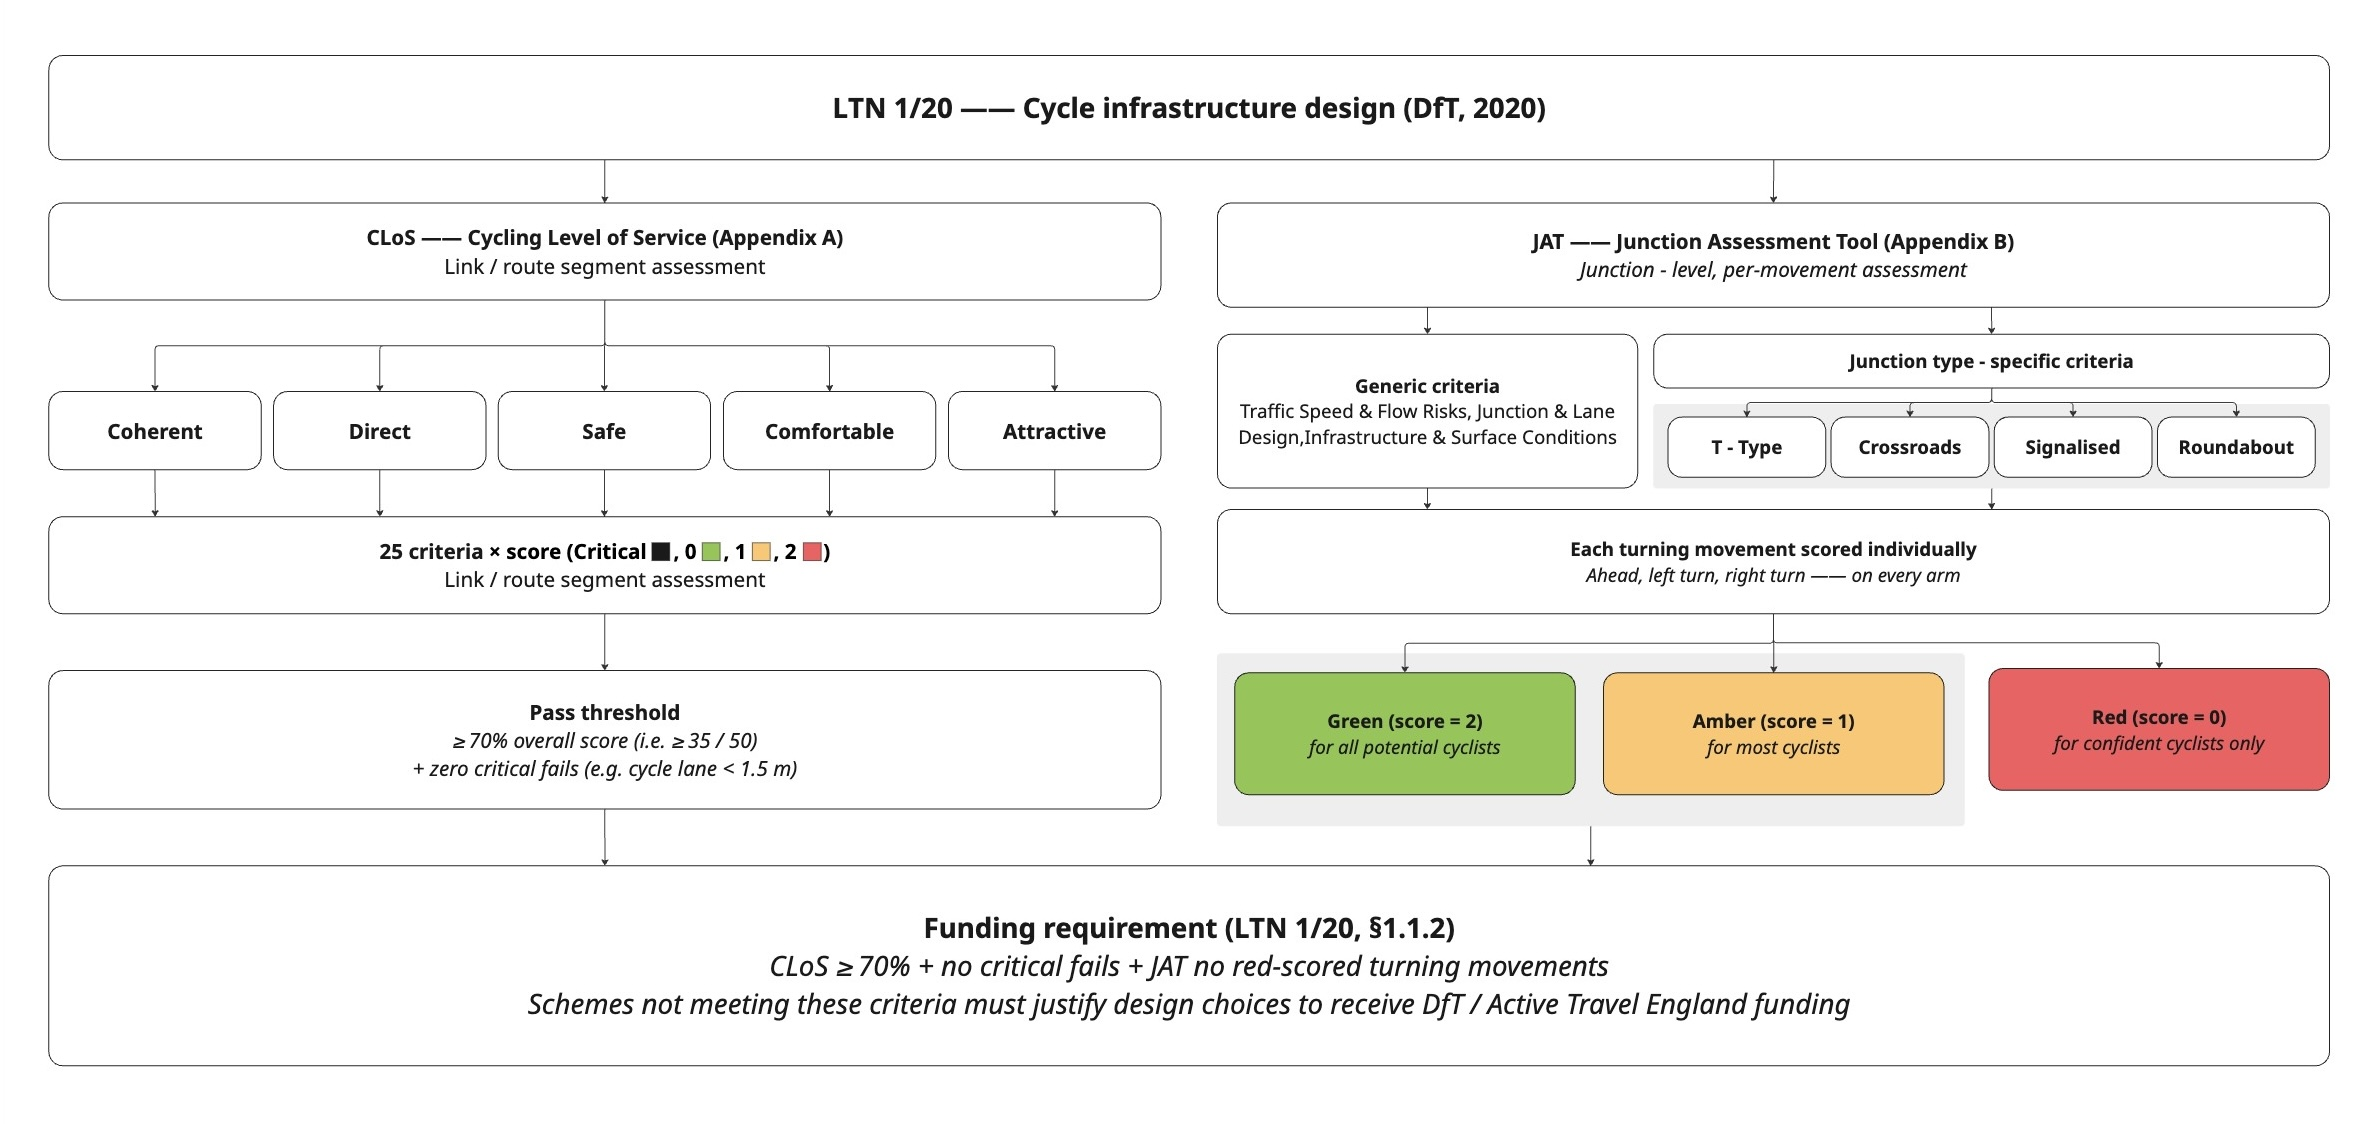
\includegraphics[width=\textwidth]{Figure/ltn.jpg}
    \caption{Structure of the LTN 1/20 evaluation framework, comprising the Cycling Level of Service (CLoS) and the Junction Assessment Tool (JAT), and their combined role in determining Active Travel England funding eligibility. Compiled by author from Department for Transport \textcite{departmentfortransport2020a}.}
    \label{fig:ltn}
\end{figure}

Despite this comprehensive coverage, LTN 1/20's evaluation tools present three structural limitations when considered as a framework for network-wide cycling assessment. Firstly, the CLoS and JAT are scheme-level audit instruments requiring on-site evaluation by trained assessors, an approach that cannot scale to the classification of all cyclable links across an urban network and that risks inconsistency where subcriteria demand qualitative judgement \parencite{hancock2024}. Secondly, the CLoS abandons the population-referenced framing that the JAT adopts for its scoring tiers, defining all 25 subcriteria in purely technical terms. This reflects a structural constraint: the subcriteria mix stress-determinant factors that do implicitly delineate population acceptability, such as motor traffic speed, volume, and segregation, with experience-quality factors that do not, such as wayfinding and cycle parking provision. Additive scoring methods of this kind are inherently compensatory, such that strong performance on one set of criteria can arithmetically offset weaknesses in another \parencite{pais2022,wang2022}; applied to CLoS, a link may therefore satisfy the 70\% threshold through strong performance on the latter while falling short on stress conditions that, though not critical failures, would nonetheless deter the majority of potential cyclists. Thirdly, while the CLoS includes coherence subcriteria that address route-level continuity, these assess attributes of individual links rather than the connectivity of the network as a whole. They cannot answer whether a cyclist can complete a journey from origin to destination entirely within tolerable traffic conditions, yet end-to-end low-stress connectivity between origins and destinations has been identified as the most fundamental determinant of whether a cycling network can attract the widest possible segment of the population \parencite{mekuria2012a,wang2016,lowry2017}.


\section{Level of Traffic Stress: Origins, Framework, and Applications }
\label{sec:lit-lts}

Where LTN 1/20 aspires to design for all from 8 to 80 but operationalises this through a broad composite of design criteria, the Level of Traffic Stress (LTS) framework \parencite{mekuria2012a} makes population acceptability the sole organising principle of its classification. Mekuria et al. operationalised this by adapting \citeauthor{geller2009}'s (\hyperlink{cite.geller2009}{\citeyear{geller2009}}) four-part population typology, the "strong and fearless," "enthused and confident," "interested but concerned," and "no way, no how," validated by \textcite{dill2013}, into an infrastructure classification. They subdivided Geller's "interested but concerned" to distinguish children from adults, yielding four LTS levels each anchored to a distinct population group: LTS 1 corresponds to children, demanding the greatest separation from traffic; LTS 2 to the mainstream "interested but concerned" adult majority, with criteria anchored to Dutch facility standards; LTS 3 to the "enthused and confident," comfortable with moderate traffic interaction; and LTS 4 to conditions tolerable only by the "strong and fearless" (Table~\ref{tab:lts-levels}). The "no way, no how," who would not cycle regardless of provision, have no corresponding level. To classify segments, LTS draws on the small number of road characteristics most directly associated with cycling stress, notably motor traffic speed, facility type and width, and the nature of intersection approaches and crossings, using readily observable attributes such as the number of traffic lanes as a proxy for variables like traffic volume that are rarely available at network scale \parencite{mekuria2012a,furth2016,furth2018,bearn2018}. Classification follows a non-compensatory rule: a segment's LTS is determined by its worst-performing attribute, so that a single high-stress condition is sufficient to determine the classification regardless of other favourable characteristics.

\begin{table}[htbp]
  \centering
  \caption{Level of Traffic Stress classification and corresponding population groups.}
  \label{tab:lts-levels}
  \begin{tabularx}{\textwidth}{l X}
    \toprule
    \textbf{LTS Level} & \textbf{Population Group and Description} \\
    \midrule
    LTS 1 & Suitable for almost all cyclists, including children cycling independently \\
    LTS 2 & Tolerable to the mainstream adult population; anchored to Dutch design standards proven to attract broad demographic participation \\
    LTS 3 & Tolerable to experienced cyclists who prefer dedicated space but accept moderate traffic interaction \\
    LTS 4 & Tolerable only to the strong and fearless riders willing to integrate with fast or heavy traffic \\
    \bottomrule
  \end{tabularx}
\end{table}

The original LTS framework proposed systematic network connectivity measures based on the population-anchored classification, quantifying the share of origin-destination pairs connected at each stress threshold and demonstrating how targeted gap closures can substantially multiply low-stress connectivity \parencite{mekuria2012a,furth2016}. This approach has since been widely adopted: a scoping review by \textcite{schon2024} identified 25 studies employing LTS to classify network links by stress level, primarily to measure cumulative accessibility by quantifying destinations reachable via low-stress links within defined distance or time thresholds \parencite{murphy2019,wasserman2019,gehrke2025}. Beyond cumulative measures, LTS-based analysis has been used to evaluate job accessibility through detour-ratio methods that permit travel on higher-stress links when low-stress routing is substantially longer \parencite{furth2016,lowry2017,cabral2019}, to assess transport equity by linking low-stress connectivity to socioeconomic indicators \parencite{tucker2018,kent2019}, and to identify network barriers and prioritise infrastructure investment \parencite{lowry2017,putta2019}. Collectively, LTS modelling and network filtering have become the dominant approaches in cycling accessibility and equity research \parencite{louro2026}.

Two limitations constrain the applicability of existing LTS implementations to the UK context. Firstly, all published criteria were calibrated to North American road design conventions, speed regimes, and infrastructure types, and no LTS classification grounded in UK design standards has been developed systematically. Although the framework has been applied to British cities \parencite{cervero2019,jeong2025}, these implementations relied on simplified criteria derived from North American conventions rather than national design guidance. Secondly, the progressive simplification of the original criteria for network-scale application has produced considerable methodological divergence, with \textcite{harvey2024} finding substantial disagreement across seven LTS methods applied to the same cities, underscoring the sensitivity of results to variable selection and threshold definitions. These two limitations motivate the approach taken in this study: rather than adapting any single North American LTS variant, the classification is grounded in LTN 1/20, a single national design standard that provides both the threshold structure and the population-acceptability logic needed to anchor an LTS classification to English conditions.


\section{Growing Fragmented Cycling Networks}
\label{sec:lit-networkgrowth}

Cycling networks in most cities remain sparse and fragmented \parencite{schoner2014,szell2022,reggiani2023}, so how they should expand, and in what order, is a live planning question. Network growth simulation addresses this by modelling expansion as the sequential addition of edges under a selection rule, generating investment trajectories whose connectivity outcomes can be compared \parencite{barthelemy2009,xie2009,szell2022}. Approaches to cycling network growth simulation can be divided by direction of construction: forward approaches iteratively add edges, either expanding from an existing network by bridging disconnected components \parencite{nateraorozco2020}, growing from scratch around topologically central seed points \parencite{szell2022}, or prioritising segments on the street network by potential routed cycling demand \parencite{mahfouz2023}. Inverse approaches begin from an idealised complete network and greedily remove the least important edges to generate budget-indexed subnetworks \parencite{steinacker2022}. Both directions can incorporate topological centrality \parencite{szell2022} or cycling demand to weight edge importance \parencite{steinacker2022,mahfouz2023}. A recurring finding is that how a fragmented network is grown matters as much as how much is built. \textcite{nateraorozco2020} show across fourteen cities that small, targeted investments connecting disconnected components rapidly consolidate a bicycle network, far outperforming random, uncoordinated addition, while \textcite{szell2022} find that uninformed growth needs several times the investment of a flow-based strategy before a connected network emerges. 

These studies operate on networks defined by infrastructure presence, in which an edge either belongs to the cycling network or does not, and they deploy growth simulation to identify an optimal expansion sequence. Neither feature carries over to a stress-classified network, where the object of investment is the upgrading of existing high-stress links, and low-stress conditions arise as much from quiet residential streets as from dedicated facilities.  

\section{Research Gap and Questions}
\label{sec:lit-gaprq}

The preceding review establishes three gaps at the intersection of design standards, network assessment, and investment planning. First, while LTN 1/20 provides the most comprehensive national design standard for cycling infrastructure in England, its evaluation instruments remain confined to scheme-level audit. The CLoS's compensatory scoring obscures the population-referenced acceptability that the standard's ``cycling for all'' principle implies, and neither the CLoS nor the JAT can assess whether compliant schemes cohere into a network that connects origins to destinations at tolerable stress levels (Section~\ref{sec:lit-ltn}), despite end-to-end low-stress connectivity being the most fundamental determinant of a network's capacity to attract the wider population \parencite{mekuria2012a,lowry2017}.

Second, the LTS framework supplies precisely the network-level, population-anchored logic that LTN 1/20's instruments lack, yet no published implementation is grounded in UK design standards. Existing applications to British cities rely on simplified adaptations of North American criteria \parencite{cervero2019,jeong2025}, and applied practice inherits further weaknesses from the Conveyal lineage: undirected max-propagation of junction stress and the absence of any treatment of roundabouts, a junction form both prevalent in the UK and associated with elevated cyclist risk (Section~\ref{sec:lit-lts}). The recent completion of the OS NGD Transport Cycle Lane collection removes the principal data barrier to a standards-grounded classification, but as a newly released dataset its completeness and reliability have not been independently assessed.

Third, the network growth literature demonstrates that the sequence of investment shapes connectivity outcomes as strongly as its volume, but existing simulations operate on networks defined by infrastructure presence, in which edges are added rather than upgraded (Section~\ref{sec:lit-networkgrowth}). Whether these findings transfer to a stress-classified network, where low-stress conditions arise as much from quiet streets as from dedicated facilities and the investment problem is one of reclassifying existing high-stress links, remains untested.

These gaps motivate the overarching aim of this dissertation: to develop and apply a network-level cycling infrastructure assessment grounded in English design standards. Three research questions structure the study:

\begin{description}
  \item[\textnormal{RQ1.}] How can the design criteria of LTN 1/20 be operationalised into a directed, network-scale Level of Traffic Stress classification, including junction and roundabout assessment, using OS NGD Transport data?
  \item[\textnormal{RQ2.}] To what extent does the West Midlands cycling network deliver the connected, low-stress conditions that LTN 1/20's ``cycling for all'' principle requires, for the population groups the standard identifies?
  \item[\textnormal{RQ3.}] How do alternative strategies for upgrading high-stress links compare in their capacity to improve low-stress network connectivity?
\end{description}
